\documentclass{beamer}
\usepackage{framed}

\usepackage{graphicx}

\begin{document}
%================================================%
\begin{frame}
\frametitle{2013 Exam Paper}
\large
\begin{itemize}
\item Explain briefly why the following strategy for the solution of I.P.’s
is not useful:
\end{itemize}
\begin{quote}
``\textit{Solve the L.P. relaxation then round off the components
	of the solution to the nearest integers}".
\end{quote} 
\end{frame}
%================================================%
\begin{frame}
\large
\noindent \textbf{Integer Programming by Branch and Bound} \\
\bigskip

 Consider the Integer Linear Program (IP):

\begin{figure}
\centering
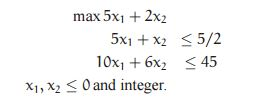
\includegraphics[width=0.7\linewidth]{Exam13-Question}
\end{figure}

%
%(b) Consider the Integer Linear Program (IP):
%max 5x1 + 2x2
%5x1 + x2 \leq 5/2
%10x1 + 6x2 \leq 45
%x1, x2 \leq 0 and integer.
\end{frame}
%================================================%
\begin{frame}
\frametitle{2013 Exam Paper}
\large
\vspace{-1cm}
\begin{figure}
\centering
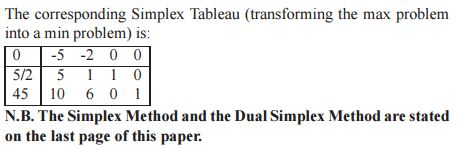
\includegraphics[width=1.1\linewidth]{Exam13-0}

\end{figure}

\end{frame}

%================================================%
\begin{frame}
\frametitle{2013 Exam Paper}
\large
\begin{itemize}
\item[(i)] Apply one iteration of the Simplex Method and show that the Simplex
Tableau now takes the form: 
\end{itemize}

\begin{figure}
\centering
\includegraphics[width=0.7\linewidth]{exam13-a}

\end{figure}

\end{frame}
%================================================%
\begin{frame}
\frametitle{2013 Exam Paper}
\large
Initial Tableau
\begin{figure}
\centering
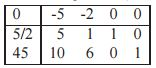
\includegraphics[width=0.4\linewidth]{exam13-0a}
\end{figure}

\begin{itemize}
\item Indicator Row at top of tableau. Pick the lowest (i.e most negative)  value. (i.e.-5)
\item This is our Pivot Column.
\item To pick the Pivot Row, compute the ratio of value in the pivot column to the ``\textit{barrier column}" (i.e. the first column) \\ (barrier column value is numerator)

\end{itemize}	


\end{frame}
%================================================%
\begin{frame}
	\frametitle{2013 Exam Paper}
	\large
	\begin{itemize}
\item Pick the row with the lowest ratio. \bigskip
{ 
\Large
\begin{itemize}
\item $\frac{5/2}{5} =0.5 $ Lowest - Pick this Row \bigskip
\item $\frac{45}{10} =4.5 $ \bigskip
\end{itemize}
}\item Pivot Point is intersection of pivot column and pivot row.
\end{itemize}	
\noindent \textbf{Elementary Row Operations}
\begin{itemize}
\item Divide Pivot Row by value of Pivot Point (Pivot Point should become 1)
\item Perform EROs such that other values on pivot column become 0.
\end{itemize}
	
	
\end{frame}
%================================================%
\begin{frame}
	\frametitle{2013 Exam Paper}
	\large
	\begin{itemize}
		\item  You should end up with this tableau
	\end{itemize}
	
	\begin{figure}
		\centering
		\includegraphics[width=0.7\linewidth]{exam13-a}
		
	\end{figure}
	
\end{frame}
%================================================%
\begin{frame}
\frametitle{2013 Exam Paper}
\large
\noindent \textbf{Next Question}
\begin{itemize}
\item[(ii)] After a second iteration of the Simplex Method the Simplex Tableau
now takes the form: (N.B.do not perform the arithmetic!) \\ Explain why this Tableau is optimal. 
\end{itemize}

\begin{figure}
\centering
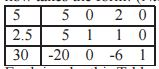
\includegraphics[width=0.7\linewidth]{exam13-b}
\end{figure}

Look at the top row (i.e. the indicator row.) All values on indicator row are positive. This is our main stopping condition.

\end{frame}
\begin{frame}
\frametitle{2013 Exam Paper}
\large
\noindent \textbf{Important:} When the two-phase Simplex method stops and all the artificial variables have value = 0, we can remove the artificial variables and remaining variables will form a feasible solution for the original LP problem
\end{frame}
\begin{frame}
\frametitle{2013 Exam Paper}
\large
Which Columns have 0 or 1 only in their column?
\begin{itemize}
	\item $x_1$ : 5 and -20 N0
	\item $x_2$ : Yes
	\item $s_1$ : 1 and -6 NO
	\item $s_2$ : Yes
\end{itemize}
Set values to zero, if this condition is not met. $x_1=0$,$s_1=0$.\\ \bigskip
Solve for the other values.\\
Pivot Row: $2.5 = 5x_1 + x_2 + s_1 + 0s_2$ \\
Necessarily $x_1$ and $s_1$ = 0 :  $2.5 =  x_2 + 0s_2$ \\
By Inspection $x_2=2.5$ \\
Solution : (0,2.5)	\\
\end{frame}
%================================================%
\begin{frame}
\frametitle{2013 Exam Paper}
\large
\begin{itemize}
\item[(iii)] Explain why the solution to the LP Relaxation of the IP is $x_1 = 0, x_2 = 2.5$ and why we must now branch on $x_2$ and what are the
two branches? 
\end{itemize}
\bigskip
\noindent  \textbf{Remarks}
Solution already provided.\\
$x_1$ has integer solution.\\
$x_2$ has none-integer solution. \\ Apply constraints using floor and ceiling function of $x_2$.\\
\bigskip 
\textbf{Branches:}  $x_2 \leq 2$ and $x_2 \geq 3$.\\
\end{frame}

\begin{frame}
\frametitle{2013 Exam}
	\large
	\begin{description}
		\item[A.] First show that the basic variable x2 may be expressed in
		terms of the non-basic variables $x_1$ and $x_3$ (also known as s1) as:
		\[x2 = 2.5 - 5x1 - x3. \]
		\item[B.] Substitute this expression for x2 into the $S_0$ branch constraint
		and show that it takes the form \[-5x_1 - x_3 + s = -0.5.\] 
	\end{description}
\textit{(Discussed Previously, but slack variable denoted with $s_1$ rather than $x_3$)}\\ \bigskip
%
\textit{(The
variable $s$ is the slack variable for the constraint $x_2 \leq 2$.) }
\end{frame}
%================================================%



%================================================%
\begin{frame}
\frametitle{2013 Exam}
\large
\begin{description}
	\item[C.] 
Show that the Simplex Tableau with the addition of this constraint
takes the form: 
\end{description}
\begin{figure}
\centering
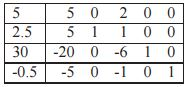
\includegraphics[width=0.7\linewidth]{exam13-c}

\end{figure}

\end{frame}
%================================================%
\begin{frame}
	\frametitle{2013 Exam}
	\large
	\begin{itemize}
		\item[(v)] Explain why this tableau is optimal but infeasible. 
	\end{itemize}
	
	
	\begin{figure}
		\centering
		\includegraphics[width=0.7\linewidth]{Exam13-c}
	\end{figure}
	
\end{frame}
\begin{frame}
	\frametitle{2013 Exam Paper}
	\large
\noindent \textbf{Important} If an LP is infeasible, then the two-phase Simplex method will stop with a solution where some slack variable has a negative value
\\
\begin{framed}
\textbf{Key Indicator:}  Infeasibility is evident when there is a negative value in the barrier column when the tableau meets the stopping condition (i.e. the indicator row shows all positive)
\end{framed}
Solve for all values on tableau of previous slide.
\end{frame}
%================================================%
\begin{frame}
\frametitle{2013 Exam}
\large
\noindent \textbf{Dual Simplex Method}
\begin{itemize}
% \item[(v)] Explain why this tableau is optimal but infeasible. 
\item[(vi)] Apply one iteration of the Dual Simplex Method (DSM) to this
tableau and show that the Simplex Tableau now takes the form: 
\end{itemize}


\begin{figure}
\centering
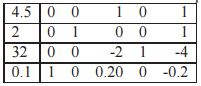
\includegraphics[width=0.7\linewidth]{Exam13-d}
\end{figure}

\end{frame}
%================================================%
\begin{frame}
\frametitle{2013 Exam}
\large
\begin{itemize}
\item[(vii)] Is this tableau LP optimal? Is it integer feasible? Explain. What
is the solution to this LP relaxation? 1
\item[(viii)] What branching should you now make?
\end{itemize}
\end{frame}
%================================================%
\begin{frame}
\frametitle{2013 Exam}
\large
\begin{itemize}
\item[(ix)] Having chosen a suitable branching, explain why the new tableau
for the left-hand branch ($x_1 = 0$) is:
\end{itemize}

\begin{figure}
\centering
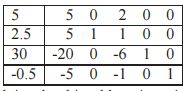
\includegraphics[width=0.7\linewidth]{Exam13-PartC}

\end{figure}

\end{frame}
%================================================%
\begin{frame}
\frametitle{2013 Exam}
\large
\begin{description}
\item[A.] What row and column is selected for pivoting with DSM? 
\item[B.] Check that, after pivoting with DSM, x1 and x2 remain basic
with x1 = 0 and x2 = 2. (\textit{No need to update the full tableau,
just the top left-hand element and the second-last element in
the the left-hand column.}) and hence find the integer optimal
value of z? 
\end{description}
\end{frame}
%================================================%
\end{document}
